\section{Motivation}

\begin{frame}{MR-to-Text}
    \begin{center}
        \begin{tikzpicture}
            \node[anchor=north west] at (0,1.0)
                {\large \textbf{Input: Meaning Representation (MR)}};
            \only<1-6>{
                \node[anchor=north west] (mr) at (0,0) 
                    {$\left[\!\!\!\left[ \begin{array}{l} 
                        \textsc{Inform} \\ 
                        \textrm{name=Aromi} \\ 
                        \textrm{eat\_type=coffee shop} \\ 
                        \textrm{area=city centre} \\ 
                    \end{array}\right]\!\!\!\right]$  };        
            }
            \only<7>{
                \node[anchor=north west] (mr) at (0,0) 
                    {$\left[\!\!\!\left[ \begin{array}{l} 
                        \textsc{Inform} \\ 
                        \textbf{\color{Red}name=Aromi} \\ 
                        \textbf{\color{Green}eat\_type=coffee shop} \\ 
                        \textbf{\color{Blue}area=city centre} \\ 
                    \end{array}\right]\!\!\!\right]$  };        
            }
            \only<2>{
                \draw[line width=0.75mm,->] (mr.south) -- (2.4,-3.5);

                \node[anchor=north west] (out) at (0,-4.0) 
                    {\large  \textbf{Output: Natural Language Utterance}};
                \node[anchor=north west,draw] (utt) at (0,-5.0) 
                    {\Large\textrm{For coffee in the city centre, try Aromi.}};
            }
            \uncover<7>{
                \draw[line width=0.75mm,->] (mr.south) -- (2.65,-3.5);

                \node[anchor=north west] (out) at (0,-4.0) 
                    {\large  \textbf{Output: Natural Language Utterance}};
                \node[anchor=north west,draw] (utt) at (0,-5.0) 
                {\Large\textrm{{\color{Green}\uline{\textbf{For coffee}}} 
                {\color{Blue}\uline{\textbf{in the city centre,}}} {\color{Red}\textbf{\uline{try Aromi.}}}}};
            }

    \uncover<3-5>{

        \node[anchor=north west,draw=mLightBrown,line width=0.5mm] (inform) at (0.43+0.05,-0.103) {\phantom{\textsc{Inform}}};
        \setbeamercolor{block title}{bg=mLightBrown,fg=white}
        \node[anchor=north west,text width=5cm,inner sep=0,outer sep=0] (da) at (5.0, -0.103) 
        {\vspace{-7.3pt}\begin{block}{Dialogue Act} 
                Goal/intent of the utterance
            \end{block}};
        \node[anchor=north west] (dafake) at (5.0,-0.103) {\phantom{\textsc{Inform}}};
        \draw[mLightBrown,thick] (inform.east) -- (dafake.west);
    }

            \uncover<4-5>{
                \node[anchor=north west,draw=Green,
                      line width=0.5mm,inner sep=0.8mm] (et) at (0.49,-1.248) 
                    {\phantom{\textrm{eat\_type}}};

                    \node[anchor=north west,line width=0.5mm,inner sep=0.8mm] 
                        (etfake1) at (-0.25,-1.248)  
                        {\phantom{\textrm{eat\_type}}};

                    \node[anchor=north west,line width=0.5mm,inner sep=0.8mm] 
                        (etfake2) at (-0.25,-3.25)  
                        {\phantom{\textrm{eat\_type}}};

                    \node[anchor=north west,line width=0.5mm,inner sep=0.8mm] 
                        (etfake3) at (0.25,-3.25)  
                        {\phantom{\textrm{eat\_type}}};

                \draw[Green,thick] (et.west) -- (etfake1.west) 
                    -- (etfake2.west) -- (etfake3.west);

                \setbeamercolor{block title}{bg=Green,fg=white}
        \node[anchor=north west,text width=4.2cm,inner sep=0,outer sep=0] (attr) at (0.0, -3.0) 
            {\begin{block}{Attributes} unordered, determines the semantics 
                of the MR\end{block}};
            }
            \uncover<5-5>{
                \node[anchor=north west,draw=VioletRed,line width=0.5mm]
                    (cc) at (1.50,-1.772) {\phantom{\textrm{city centre}}};
                \setbeamercolor{block title}{bg=VioletRed,fg=white}
                \node[anchor=north west,text width=4.0cm,inner sep=0,
                      outer sep=0] 
                    (val) at (5.0, -3.0) 
                    {\begin{block}{Attribute Values} 
                        \begin{itemize}
                            \item categorical \\ 
                            \item list-valued \\ 
                            \item free-text 
                        \end{itemize}\end{block}};

                \node[anchor=north west] (ccfake1) at (9.5, -1.772) 
                    {\phantom{\textrm{city centre}}};
                \node[anchor=north west] (ccfake2) at (9.5, -3.25) 
                    {\phantom{\textrm{city centre}}};
                \node[anchor=north west] (ccfake3) at (8.5, -3.25) 
                    {\phantom{\textrm{city centre}}};

                \draw[VioletRed,thick] (cc.east) -- (ccfake1.west) 
                    -- (ccfake2.west) -- (ccfake3.west);
            }
        \end{tikzpicture}
    \end{center}
\end{frame}



\begin{frame}{NLG as Seq2Seq}
   
    \resizebox{\textwidth}{!}{
    \begin{tikzpicture}
   \uncover<1-3>{
       \node[align=left,text width=10cm,anchor=north west] at (0,0) {\texttt{{\color{mLightBrown}\# Input}\\x = ?}};
   }

   \uncover<4>{
       \node[align=left,text width=10cm,anchor=north west] at (0,0) {\texttt{{\color{mLightBrown}\# Input}\\x = [\\~\\~\\~\\~\\~\\~\\]}};
   }
   \uncover<3-4>{
       \node[anchor=west] at (0.5,-2.8) 
       {\resizebox{5.5cm}{!}{$\uncover<4>{\pi = \left(} \left[\!\!\!\left[ \begin{array}{l}
        \textsc{Inform}\\
        \textrm{name=Aromi}\\
        \textrm{eat\_type=coffee shop}\\
        \textrm{area=city centre}\\
    \end{array}\right]\!\!\!\right]\uncover<4>{\right)}$ }};

   }
   \uncover<5->{
       \node[align=left,text width=10cm,anchor=north west] at (0,0) {\texttt{{\color{mLightBrown}\# Input}\\x = [\\
                    ~~~~"<start>",\\
                ~~~~"inform",\\
                ~~~~"name=Aromi",\\
                ~~~~"eat\_type=coffee shop",\\
                ~~~~"area=city centre",\\
                ~~~~"<stop>"\\
            ]\\~
   }};
}
   \uncover<1>{
       \node[align=left,text width=5.75cm,anchor=north west] at (6.2,0) {\texttt{{\color{mLightBrown}\# Output}\\y = ?}};
   }
   \uncover<2->{
         \node[align=left,text width=5.75cm,anchor=north west] at (6.2,0) {\texttt{{\color{mLightBrown}\# Output}\\y = [\\ 
                    ~~~~"<start>",\\ 
                    ~~~~"for",\\
                    ~~~~"coffee",\\
                    ~~~~"in",\\
                    ~~~~"the",\\
                    ~~~~"city",\\
                    ~~~~"centre",\\ 
                    ~~~~",",\\
                    ~~~~"try",\\
                    ~~~~"aromi",\\
                    ~~~~".",\\
                    ~~~~"<stop>"\\
                ] \\ ~
   }};
   }

   \draw[mLightBrown!30] (6.2,0) -- (6.2,-8.15);
   \draw[mLightBrown!30] (0,0) -- (0,-4.85);
    \end{tikzpicture}
}
\end{frame}


\begin{frame}{NLG as Seq2Seq}

    \begin{center}
    \begin{tikzpicture}

        \node[draw=black,text width=3.5cm,minimum height=1.5cm,align=center] (enc) at (1.5,2) {Encoder};
        \node[draw=black,text width=3.5cm,minimum height=1.5cm,align=center] (dec) at (7.5,2) {Decoder};

        \draw[->] (enc.east) -- (dec.west);

        \node (x1) at (0,0) {$x_1$};
        \node (x2) at (1,0) {$x_2$};
        \node (x3) at (2,0) {$\cdots$};
        \node (xn) at (3,0) {$x_m$};


        \draw[->] (x1.north) -- +(0,1);
        \draw[->] (x2.north) -- +(0,1);
        \draw[->] (xn.north) -- +(0,1);

        \node (y1) at (6,0) {$y_1$};
        \node (y2) at (7,0) {$y_2$};
        \node (y3) at (8,0) {$\cdots$};
        \node (yn) at (9,0) {$y_{n-1}$};
        \draw[->] (y1.north) -- +(0,1);
        \draw[->] (y2.north) -- +(0,1);
        \draw[->] (yn.north) -- +(0,1);

        \node (o1) at (6,4) {$y_2$};
        \node (o2) at (7,4) {$y_3$};
        \node (o3) at (8,4) {$\cdots$};
        \node (on) at (9,4) {$y_{n}$};

        \draw[->] (o1)+(0,-1.25) -- (o1.south);
        \draw[->] (o2)+(0,-1.25) -- (o2.south);
        \draw[->] (on)+(0,-1.25) -- (on.south);

    \end{tikzpicture}
    \end{center}

Encoder/Decoder is either a GRU w/ Attention or Transformer.

\end{frame}


\begin{frame}{Controllable Generation}
            Surface realization order is determined by encoder, not the decoder language model.

~\\
            
        \begin{center}
    \resizebox{0.95\textwidth}{!}{
    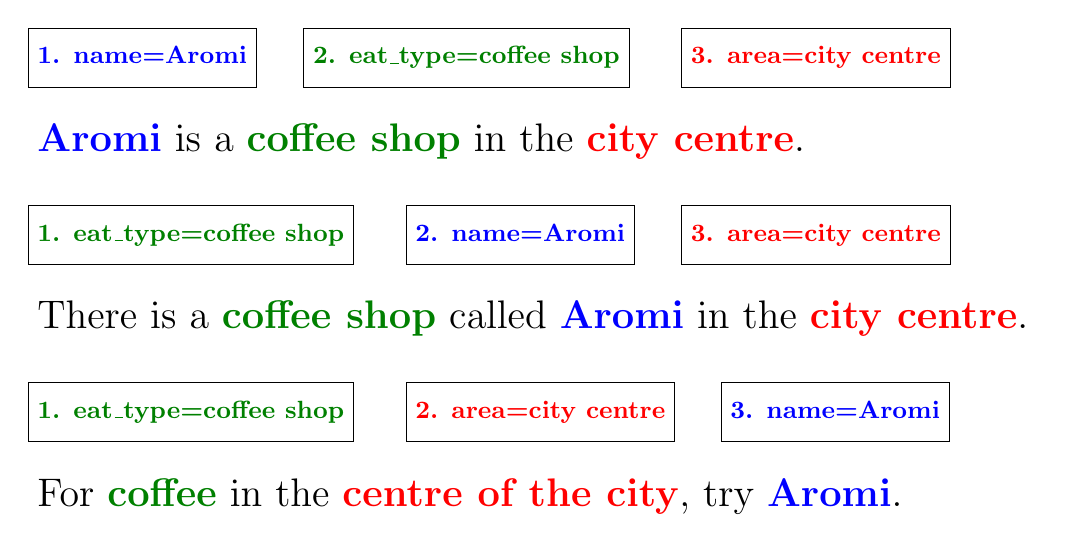
\begin{tikzpicture}
        \uncover<2->{
            \node[draw,anchor=north west,text=Blue,minimum height=0.75cm] at (0,0) {\small \textbf{1. name=Aromi\vphantom{p}}} ;
            \node[draw,anchor=north west,text=Green,minimum height=0.75cm] at (3.5,0) {\small \textbf{2. eat\_type=coffee shop}} ;
            \node[draw,anchor=north west,text=Red,minimum height=0.75cm] at (8.30,0) {\small \textbf{3. area=city centre}};
        \node[anchor=north west] at (0,-1.1) {\Large {\color{Blue}\uline{\textbf{Aromi}}} is a {\color{Green}\uline{\textbf{coffee shop}}} in the {\color{Red}\uline{\textbf{city centre}}}.};
    }
    \uncover<3->{
        \node[draw,anchor=north west,text=Green,minimum height=0.75cm] 
            at (0,-2.25) {\small \textbf{1. eat\_type=coffee shop}};
        \node[draw,anchor=north west,text=Blue,minimum height=0.75cm] 
        at (4.80,-2.25) {\small \textbf{2. name=Aromi\vphantom{p}}};
        \node[draw,anchor=north west,text=Red,minimum height=0.75cm] 
            at (8.3,-2.25) {\small \textbf{3. area=city centre}};
        \node[anchor=north west] at (0,-3.35) {\Large There is a {\color{Green}\uline{\textbf{coffee shop}}} called {\color{Blue}\uline{\textbf{Aromi}}} in the {\color{Red}\uline{\textbf{city centre}}}.} ;
    }
    \uncover<4->{
        \node[draw,anchor=north west,text=Green,minimum height=0.75cm] at (0,-4.5) {\small \textbf{1. eat\_type=coffee shop}};
        \node[draw,anchor=north west,text=Red,minimum height=0.75cm] at (4.8,-4.5) {\small \textbf{2. area=city centre}};
        \node[draw,anchor=north west,text=Blue,minimum height=0.75cm] at (8.8,-4.5) {\small \textbf{3. name=Aromi\vphantom{p}}} ;
        \node[anchor=north west] at (0,-5.6) {\Large For {\color{Green}\uline{\textbf{coffee}}} in the {\color{Red}\uline{\textbf{centre of the city}}}, try {\color{Blue}\uline{\textbf{Aromi}}}.} ;
    }



    \end{tikzpicture}
}
        \end{center}

\end{frame}


\begin{frame}{Controllable Generation}


    Controllable generation will allow us to 
    \begin{itemize}
        \item implement more cognitively plausible
    discourse structuring models, and 
\item more easily generate diverse outputs.
    \end{itemize}
    


\end{frame}


\begin{frame}{Questions}
\begin{itemize}
\item Can you make an arbitrary sequence2sequence model controllable?
\item Are there differences in systematicity between recurrent models or
transformers?
\item What about large pretrained models?
\item How systematic is a controllable sequence2sequence model?
\item Can we improve systematicity with data-augmentation?
\item How do different linearization strategies compare on faithfulness?
\end{itemize}
\end{frame}
